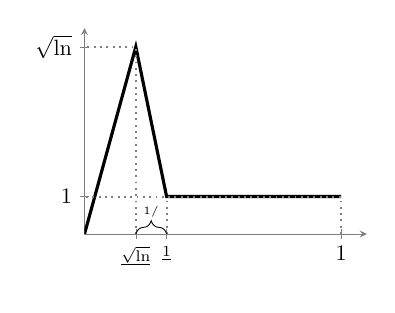
\begin{tikzpicture}[scale=0.8, transform shape]
\begin{axis}[
axis line style=gray,
axis lines=middle,
xtick={0, 0.2, 0.32, 1},
ytick={0, 1, 5},
xticklabels={0, $\frac{\sqrt{\ln\constantH}}{\constantH}$, $\frac{1}{\val\primed}$, 1},
yticklabels={0, 1, ${\sqrt{\ln\constantH}}$},
xmin=0,xmax=1.1,ymin=-0.0,ymax=5.5,
width=0.5\textwidth,
height=0.4\textwidth,
samples=1000]


\addplot[black!100!white, line width=0.5mm] (0, 0) -- (0.2, 5) -- (0.32, 1) -- (1, 1);


\addplot[dotted, gray, line width=0.3mm] (1, 0) -- (1, 1) -- (0, 1);
\addplot[dotted, gray, line width=0.3mm] (0.2, 0) -- (0.2, 5) -- (0, 5);
\addplot[dotted, gray, line width=0.3mm] (0.32, 0) -- (0.32, 1);

\draw[decorate,decoration={brace,amplitude=6pt}] (0.2,0) -- (0.32,0) node[midway,above=4pt] {\tiny $1/\constantH$};


\end{axis}

\end{tikzpicture}